\section{Objectives}
Implement the Lab 22 four-to-one MUX from PDF pages 88--90, including both handout architectures, a faster TG design, and delay/power versus load.

\section{Specification Mapping}
S denotes simulated checks; D denotes analytical discussion.

\small\begin{longtable}{p{.46\linewidth}p{.30\linewidth}p{.15\linewidth}}\toprule
Requirement and PDF pages & Deck / check & Status \\ \midrule\endhead
Fig.22.3 TG/static CMOS, 10fF (88--89) & D01; D02/C0 & S \\
Delay, power and device counts (89) & D02; source probes & S+D \\
Design a faster TG MUX (89) & Wide unbuffered tree & S; data path \\
Load dependence of all three MUXes (90) & D02; 1--500fF & S \\
Complete 4-to-1 truth table & D01; 64 codes & S \\
\bottomrule\end{longtable}\normalsize


\section{Circuit and Design Derivation}
\[Y=\overline S_1\overline S_0A_0+\overline S_1S_0A_1+S_1\overline S_0A_2+S_1S_0A_3.\]
The lecture TG circuit uses an input inverter and two series TGs per path, followed by one shared output inverter. Static CMOS uses four NAND3 gates and one NAND4. The new design is a two-level binary tree with six TGs, each at eight times unit width, directly driving the output without output inverters. All L are 0.25 $\mu$m, with unit $W_p/W_n=3.6/1.8\,\mu$m; stacked NAND NMOS widths scale with stack length. Each architecture adds two select inverters. The new tree has no gain restoration and depends on upstream data drive; fewer devices do not imply smaller total area.

Zero-volt probes at every data input separately measure input energy, preventing supply-only power from hiding the unbuffered tree's cost. Supply+data still excludes ideal select-source energy and does not model a real upstream driver.

\section{Simulation Setup}
The model is supplied separately on the user's computer. These are 1 V, 27 $^\circ$C teaching conditions; the handout's old-process 2.5 V numbers are not pass thresholds. Actual PrimeSim HSPICE S-2021.09 runs use \texttt{accurate}, \texttt{runlvl=5} and \texttt{.print/.measure} data. Every \texttt{.alter} resets baseline parameters and temperature. All cases completed without errors or failed measurements; model and convergence notices may remain. Public netlists retain only \texttt{* MODEL\_SETUP\_REQUIRED}, with no model path. Full data are under the lab's \texttt{results/}; large files are split by deck and indexed by \texttt{simulation\_data.json}.

Two decks contain six cases. D01 enumerates all 64 data/select combinations, 2 ns each, checking outputs at 80\% of each slot against 0.1/0.9 V thresholds. D02 holds select=00, drives A0 with 20 ps edges and a 10 ns period, and loads 1/10/50/100/500 fF, with at most 1 ps steps. Delay uses A0-to-output 50\% crossings; this is not worst-case select delay.

\section{Results and Specification Checks}
\begin{center}\small\begin{tabular}{lrrr}\toprule
Architecture & MOS core/all & $t_{rise}$ (ps) & $t_{fall}$ (ps) \\ \midrule
Lecture TG & 26/30 & 381.86 & 560.61 \\
Static CMOS & 32/36 & 230.90 & 364.48 \\
Wide TG tree & 12/16 & 52.16 & 92.85 \\
\bottomrule\end{tabular}\end{center}
\begin{center}\small\begin{tabular}{lrrr}\toprule
Architecture & $P_{supply}$ ($\mu$W) & $P_{data}$ ($\mu$W) & $P_{sum}$ ($\mu$W) \\ \midrule
Lecture TG & 23.886 & 2.943 & 26.829 \\
Static CMOS & 19.060 & 2.311 & 21.371 \\
Wide TG tree & -1.720 & 66.417 & 64.698 \\
\bottomrule\end{tabular}\end{center}
\begin{center}\small\begin{tabular}{lrrr}\toprule
Load (fF) & TG max (ps) & CMOS max (ps) & Tree max (ps) \\ \midrule
10 & 560.61 & 364.48 & 92.85 \\
1 & 507.14 & 348.69 & 90.62 \\
50 & 692.41 & 413.43 & 103.46 \\
100 & 799.99 & 474.38 & 116.16 \\
500 & 1586.69 & 1426.36 & 208.96 \\
\bottomrule\end{tabular}\end{center}

\begin{figure}[!htbp]\centering
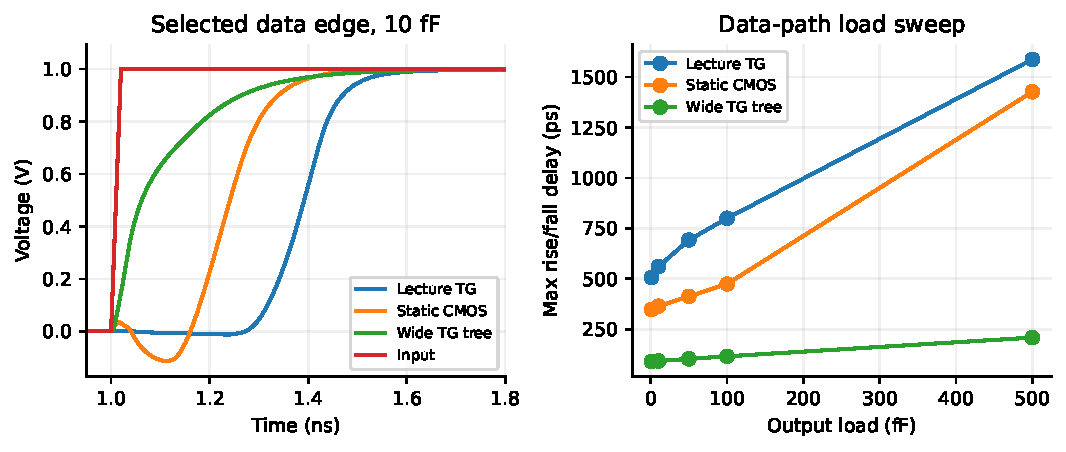
\includegraphics[width=\linewidth]{figures/mux_delay_load.pdf}
\caption{10 fF data path and load sweep. The faster tree requires the data source to supply output charging current directly.}
\end{figure}

\begin{figure}[!htbp]\centering
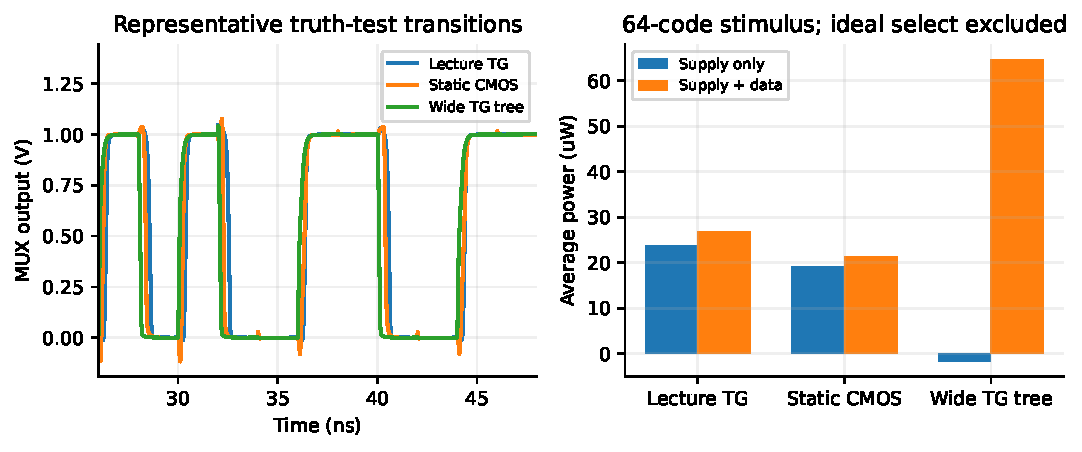
\includegraphics[width=\linewidth]{figures/mux_function_power.pdf}
\caption{Representative truth-test transitions and 64-code power. Negative supply power is net returned energy, not negative total consumption.}
\end{figure}
All three architectures pass all 64 truth-table combinations. At 10 fF, the new tree gives 52.16/92.85 ps rise/fall delay, below static CMOS at 230.90/364.48 ps, meeting the selected data-path speed goal. Yet supply+data power for the truth stimulus is 64.70 $\mu$W, above CMOS at 21.37 $\mu$W. The tree's -1.72 $\mu$W supply-only value is not an energy-saving result.

\section{Discussion}
Wider TGs lower channel resistance and removing inverters saves gate delay, but increases data/select capacitance and shifts output charging energy to the upstream source. Finite drivers, interconnect or cascaded MUXes can reduce the advantage and require regeneration. Static CMOS restores gain and provides active output drive. The original TG version provides regeneration but adds transmission delay. All delays increase with load; the ordering applies only to these sizes and input conditions.

Transition glitches and rail excursions remain visible rather than being hidden by settled truth checks. Counts exclude stimulus, loads and probes; differing widths also prevent transistor counts from representing layout area.

\section{Conclusion}
The handout circuits, faster TG design, exhaustive truth table and five loads are verified. Faster selected-data timing costs input energy and gain restoration, and is not a universal optimum for all paths or complete systems.
